\documentclass[12pt,oneside]{book}
\pagestyle{headings}

% Note that the line below could be modified to suit a
% particular system since the "geometry" package behaves
% differently in Unix, Windows and Mac, especially for the
% top margins.
% Adjust the parameter "top" (measuring the height of the
% space allocated to a header) and "headsep" (measuring
% the distance from the bottom of the header to the
% first line of text.
\usepackage[top=1.3in,left=1.5in,bottom=1in,right=1in,headsep=0.5in]{geometry}

\usepackage{setspace}
\onehalfspacing
%\doublespacing

% Headers and footers for thesis
\usepackage{fancyhdr}

\markboth{}{}
\newcommand\startchapter[1]{\chapter{#1}\thispagestyle{myheadings}}
\newcommand\startappendix[1]{\chapter{#1}\thispagestyle{myheadings}}
\newcommand\startfirstchapter[1]{\chapter{#1}}

% Manual addition of section to Table of Contents
\newcommand\TOCadd[1]{\newpage\phantomsection\addcontentsline{toc}{chapter}{#1}}

% Float Customization
\renewcommand{\floatpagefraction}{0.01}

% Customization of Tables of Contents and List of Figures/Tables
\usepackage{tocloft}
\renewcommand\cfttabpresnum{Table\ }
\renewcommand\cfttabnumwidth{0.75in}
\renewcommand\cftfigpresnum{Figure\ }
\renewcommand\cftfignumwidth{0.80in}
\newcommand{\HRule}{\rule{\linewidth}{0.5mm}}
% Long Table and decimal aligned columns
\usepackage{dcolumn}
\usepackage{longtable}

% Mathematics support
\usepackage{amsmath}
\usepackage{amsthm}
\usepackage{amssymb}


% Text Control
\usepackage{xspace}
\usepackage{textcase}

% Graphics
\usepackage{wasysym}
\usepackage{graphics}
\usepackage{graphicx}   % A package to allow insertion of
                        % external image files

% rohith specific packages
\usepackage[hidelinks]{hyperref}
\usepackage{xcolor}
\usepackage{textcomp}
\usepackage{listings}
\usepackage[listings, many]{tcolorbox}
\usepackage[OT1]{fontenc} 
\usepackage{color}
\usepackage{hyperxmp}


% colors
\definecolor{lightgray}{rgb}{.9,.9,.9}
\definecolor{codegreen}{rgb}{0,0.6,0}
\definecolor{codegray}{rgb}{0.5,0.5,0.5}
\definecolor{codepurple}{rgb}{0.58,0,0.82}
\definecolor{backcolour}{rgb}{0.95,0.95,0.92}

\lstdefinelanguage{JavaScript}{
  keywords={typeof, new, true, false, catch, function, return, null, catch, switch, var, if, in, while, do, else, case, break, console, const},
  keywordstyle=\color{blue},
  ndkeywords={class, export, boolean, throw, implements, import, this, for},
  ndkeywordstyle=\color{magenta},
  identifierstyle=\color{black},
  sensitive=false,
  comment=[l]{//},
  morecomment=[s]{/*}{*/},
  commentstyle=\color{codegreen}\ttfamily,
  stringstyle=\color{red}\ttfamily,
  morestring=[b]',
  morestring=[b]"
}

\lstset{
  language=JavaScript,
  backgroundcolor=\color{lightgray},
  extendedchars=true,
  basicstyle=\footnotesize\ttfamily,
  showstringspaces=false,
  showspaces=false,
  numberstyle=\footnotesize,
  numbersep=9pt,
  tabsize=2,
  breaklines=true,
  showtabs=false,
  captionpos=b
}

\lstdefinestyle{mystyle}{
    backgroundcolor=\color{backcolour},   
    commentstyle=\color{codegreen},
    keywordstyle=\color{magenta},
    numberstyle=\tiny\color{codegray},
    stringstyle=\color{codepurple},
    basicstyle=\ttfamily,
    breakatwhitespace=false,         
    breaklines=true,                 
    captionpos=b,                    
    keepspaces=true,                 
    numbers=left,                    
    numbersep=5pt,                  
    showspaces=false,                
    showstringspaces=false,
    showtabs=false,                  
    tabsize=2
}
\lstset{style=mystyle}
\lstset{escapeinside={\%*}{*)}}


%% rohith commands
\newcommand{\AIDE}{AI-supported programming}%{AI-driven development}
\newcommand{\AISE}{AI-supported software engineering}%{AI-driven software engineering}
\newcommand{\cct}{AI-supported code completion tools}
\newcommand{\cop}{GitHub Copilot}
\newcommand{\repl}{replication package at \url{todo}}

%% table wrap text helper
\newcolumntype{L}{>{\centering\arraybackslash}m{.42\linewidth}}

\begin{document}

% Front Matter
\input frontmatter/fm

\newpage

	\startfirstchapter{Introduction}
\label{chapter:introduction}
Programming is a powerful and ubiquitous problem-solving tool. Developing systems that can assist software developers or even generate programs independently could make programming more productive and accessible. 
Code completion is a feature that predicts what a software developer is trying to code and offers predictions as suggestions to the user. All modern IDEs feature intelligent code completion tools in different forms and it is used by both new and experienced software developers. Developing AI systems that can effectively model and understand code can transform these code completion tools and the way we interact with them.

Recent large-scale pre-trained language models such as \cop{}~\cite{Copilot-web} have demonstrated an impressive ability to generate code and are now able to solve programming contest style problems~\cite{empirical_eval}. 
However, software engineering is much more than writing code, it involves complex challenges like choosing the best practices, avoiding code smells, using design patterns and many more decisions before writing code. 
The scope of capabilities for \cct{} is uncertain. Identifying the nature of \cop{} capabilities when it comes to more complex challenges, i.e., \AISE{} (as opposed to development tasks, such as coding or programming problems). Delineating where \cct{} are currently best able to perform, and where more complex software engineering tasks overwhelm them is helpful in answering questions like 
Exactly which software problems can current \cct{} solve? 
If \cct{} makes a suggestion, is that suggestion accurate and optimal? Should a user intervene to correct it? But identifying these boundaries is a challenging task. In the next section, we discuss this challenge and the research opportunity that it creates as the motivation for this study.

\section{Motivation}


In this thesis, we investigate the

\section{\cct{}}




\section{Problem Statement and Research Questions}
The overarching goal of this study is to:
\begin{quote}
    Identify the boundaries of the capabilities of GitHub Copilot. Toward this goal, we compare Copilot code suggestions against well known language idioms and code smells. Additionally, we introduce a simple taxonomy of software abstraction hierarchies to show different capability levels of \cct{}. 
\end{quote}

The capabilities and the limitations of current \cct{} like Copilot are unknown, identifying the limitations of \cct{} would help the users use the tool effectively and focus more on the tasks \cct{} are shown to be not useful. 
The objective of this study is to achieve a better understanding of the areas Copilot performs better than a human and the areas where Copilot performs worse than a human. We conduct an exploratory study with the following research objectives:

\begin{enumerate}
  \item[\textbf{RQ-1: }]
  \textbf{What are the current boundaries of \cct{}?} \\
  \textbf{Approach -} We use GitHub's Copilot as a representative for \cct{}. We explore Copilot's code suggestions for code smells and usage of language idioms. We conduct additional investigation to determine the current boundaries of Copilot by introducing a taxonomy of software abstraction hierarchies where ‘basic programming functionality’ such as code compilation and syntax checking is at the least abstract level. Software architecture analysis and design is at the most abstract level. 
  
  \item[\textbf{RQ-1.1: }]
  \textbf{How do \cct{} manage programming Idioms?} \\
  \textbf{Approach -} We examine Copilot code suggestions on top 25 idioms used in open source projects sampled from work of Alexandru et al.~\cite{Alexandru2018}, which identified idioms from presentations given by renowned Python developers. We investigate how Copilot's top code suggestion compares to Python idioms from Alexandru et al.~\cite{Alexandru2018}. In addition, we report if the idiom is listed in any of the 10 viewable suggestions from Copilot.
  
  \item[\textbf{RQ-1.2: }]
  \textbf{How do \cct{} manage manage to suggest non-smelly code?} \\
\textbf{Approach -} We examine Copilot code suggestions on 25 different best practices sampled from AirBNB JavaScript coding style guide~\cite{airbnb_code}. We investigate how Copilot's top code suggestion compares to the best practices in AirBNB JavaScript coding style guide~\cite{airbnb_code}. Additionally, we report if the best practice is listed in any of the 10 viewable suggestions from Copilot. 
 
  \item[\textbf{RQ-2: }]
  \textbf{Given the current boundary, how far is it from suggesting design decisions which seem much beyond the boundary??} \\
  \textbf{Approach -} Based on our findings in RQ-1, we discuss how far current \cct{} are from the design level in our taxonomy. We look at current limitations of Copilot and provide recommendations on how to make current \cct{} reach design abstraction level. Additionally, we report on ethical considerations, explainability and control of \cct{} like Copilot. 
\end{enumerate}
\section{Contributions}
\section{Thesis Outline}



	\startchapter{Background \& Related Work}
\label{chapter:background}

\newlength{\savedunitlength}
\setlength{\unitlength}{2em}

\section{Introduction}

\section{\cct{} Journey}

\subsection{Before Copilot}

\subsection{Alternatives to Copilot}
\section{\cct{} related works}
\section{Challenges with \cct{}}
\label{challenges}
Some of these basic programming challenges have been already documented and are, we suspect, very much under consideration by the corporate teams behind Copilot and Codex. Since these tools are trained on existing software source code, and training costs are expensive, several classes of errors have been discovered, which follow from the presence of these same errors in public (training) data.

Copilot can make simple coding mistakes, such as not allowing for an empty array in a sort routine\footnote{all examples are documented in our \repl{}.}. Copilot does not understand security vulnerabilities, so it will suggest code that allows for a \textsf{log4shell} vulnerability\footnote{\url{https://www.wiz.io/blog/10-days-later-enterprises-halfway-through-patching-log4shell/}}, or common SQL injection attacks. A recent study by Pearce et al.~\cite{copilot_security} showed that approximately 40\% of the code suggested by Copilot is found to be vulnerable, when tested on 89 different scenarios for Copilot to complete.
Similarly, concerns have been raised about Copilot licence compliance and copyright violation~\cite{code_clone}; with similar input data, Copilot suggests identical code to existing code on GitHub, which may be under copyright. 

% Karampatsis et al.~\cite{github_bugs} showed that for the 1000 most popular open-source Java repositories on GitHub, there is a frequency of one single statement bug per 1600-2500 lines of code and about 33\% of all the bugs match a set of 16 bug templates. This shows that there are bugs which occur repeatedly in the public repositories of GitHub, which can make Copilot biased to suggest bug prone code over bug-free versions.
As it is trained on public data collected in May 2020 from 50 million public repositories on GitHub~\cite{copilot}, any code uploaded after that date is absent in the knowledge base of Copilot. 
% The training data for Copilot was collected in May 2020 from 50 million public repositories on GitHub~\cite{copilot}. 
%It does not have any data uploaded to GitHub after that date and any data from useful sources like documentation and Stack Overflow to improve its suggestions from commonly occurring bugs.
Any software flaws present in large numbers on GitHub will tend to dominate the learning of the model.

But these challenges are not surprising, and have straightforward fixes.
Fixes might include better data engineering and filtering, to remove known problems. This is already part of the training of these large language models, although the exact process has not been publicly disclosed. 
Similarly, it seems viable to conduct security scans or linting runs prior to making a suggestion, in order to remove obvious problems like SQL injection. 
Clone detection techniques can help find places where code violates copyright. 
Better machine learning approaches, using active learning or fine-tuning, might help learn local lessons~\cite{Menzies2013} for customization in the case of identifier naming or formatting.
In most of these cases, good tools exist already for this. 

Our belief is that while heuristic, such flaws can be fixed and will be fixed in short order. 
What we believe is harder to fix will be problems where straight-forward corrections may not exist and rules for finding problems are harder to specify than those in smell detectors or linters ~\cite{Ernst2017}.

\section{Chapter Summary}
In this chapter, we first provided some background on different language models used for \cct{} and their limitations. We reviewed early developments in \cct{} with statistical language models like N-grams. Followed by a discussion on N-gram based \cct{} and the limitations of statistical language models, resulting in using neural language models for \cct{}. We established the importance of transformers for \cct{} which is a crucial component of OpenAI's Codex Model~\cite{copilot}. To further explore the role of transformer architecture in \cct{}, we reviewed studies showing context-sensitive contextualised word representations were presented by LMs such BERT~\cite{bert}.

We then discussed GitHub Copilot, the \cct{} we would use as the basis for our study in this thesis. Additionally, we reviewed the key functionalities of Copilot.
Furthermore, we discussed some of the related works on Copilot about its usage~\cite{Vaithilingam2022} and its effectiveness in solving programming contest style problems~\cite{empirical_eval}. We concluded by introducing some of the other \cct{} that provide similar functionality like Copilot.

In the next chapters, we discuss the problems with using \cct{} like Copilot that are harder to fix and straight-forward corrections may not exist, like language idioms and code smells. 
We try to address \textbf{RQ-1} (What are the current boundaries of code completion tools) using the methodology and present our results~(Chapter~\ref{chapter:methodology}).
We then introduce a taxonomy of software abstraction hierarchy to help with finding the current boundaries of \cct{} like Copilot (Chapter~\ref{chapter:framework}). We address \textbf{RQ-2} (Given the current boundary, how far is it from suggesting design decisions?) with a discussion of the complex nature of design decisions, and the challenges with trying to use \cct{} to make design decisions.
Finally, we discuss some of the practical implications, limitations of our findings and also provide some future directions to help further research in \cct{} (Chapter~\ref{chapter:discussion}).

\setlength{\unitlength}{\savedunitlength}

	\startchapter{Code Smells}
\label{chapter:smells}

\section{Introduction}
Useful \AISE{} tools should always suggest the optimal way as its first suggestion. In this chapter, we test if \cop{} suggests the optimal way. 
We begin by explaining our approach to \textbf{RQ-1.1} (How do \cct{} manage to write non-smelly code?).

To achieve this, we conduct an exploratory study to find how often does current \cct{} suggest the optimal way in their suggestions. In section~\ref{methodology}, we describe our methodology for the two categories under study: python idioms (Section~\ref{secidioms}) and best practices in javascript (Section~\ref{bp}).
We then compare the suggestions generated by \cop{} and previous works on best practices in Python and JavaScript. We report on how many times \cop{} suggested the optimal way. 

We find that \cop{} performs poorly in suggesting the optimal way in its suggestions. Further, in section~\ref{evolution}, we provide a detailed discussion on how best practices change over time with an example from Asynchronous JavaScript and outline the difficulties of a \cct{} to keep updating its suggestions and reflect the current best practice.


\section{Methodology}
\label{smells:methodology}
In this Section, We explain the methodology we used to address \textbf{RQ-1.2} (How do \cct{} manage programming Idioms and Best Practices?), including how the best practices were sampled (Section~\ref{smells:sampling}), what was the input for copilot (Section~\ref{smells:input}) and how is the suggestion evaluated (Section~\ref{smells:evaluation}). All of the following analysis was carried out using \cop{} extension in Visual Studio Code. We use the most recent stable release of Copilot extension (version number todo) in Visual Studio Code.

\subsection{Sampling Approach}
\label{smells:sampling}
To give the best chance for \cop{} to suggest the optimal way, we sampled the top ten most frequent idioms used in open source projects. So that, \cop{} will have the optimal way more frequently in its training data. However, \cop{} is closed source and we cannot determine if the frequency of code snippet in training data affects \cop{} suggestions in any way. Research by GitHub shows that Copilot can sometimes recite from its training data in ``generic contexts"\footnote{\url{https://github.blog/2021-06-30-github-copilot-research-recitation/}}, which may lead to Licence Infringements shown in Section~\ref{challenges}. Sampling the most frequently used Idioms will also help understand if copilot can recite idioms, which is the ideal behaviour for \cct{}.

\subsection{Study Setup}

\subsubsection{Input to \cop{}}
\label{smells:input}
The input to \cop{} consisted of the idiom title as the first comment to provide context, and the input was restricted to being able to derive the ideal way from the input. This is done to ensure \cop{} is making the decision to suggest the good/bad way in its suggestions. This input style also mimics a novice user, who is unaware of the idioms and useful \cct{} should drive the novice user to use best practices.

\subsubsection{Evaluation}
\label{smells:evaluation}
We considered \cop{} suggested the optimal way if Copilot suggested the best practice in the first suggestion, In this case, we considered \cct{} like \cop{} as productivity tool and user should be saving time as opposed to writing the optimal way without using \cct{}, Scrolling through all the suggestions to deduce the optimal way defeats this purpose. For this reason, We restricted ourselves to first suggestion. However, we do note if the best practice appeared any of the top 10 suggestions currently viewable in \cop{} interface. 

\section{Results}
\subsection{Code Smells}
\label{bp}
A good \AISE{} tool should only suggest code that passes code reviews by humans. We relied on the AirBNB JavaScript coding style guide~\cite{airbnb_code}, a widely used coding style and code review standard. 

The AirBNB JavaScript coding style guide contains a variety of best practices. 
Since, we are testing \cop{} for widely accepted practices and not project specific styling in JavaScript. We chose practices that were closer to design level rather than code level (e.g., logging practices rather than trailing comma use in Javascript).

Using the methodology described in Section~\ref{smells:methodology}, we picked 10 best practices in JavaScript from AirBNB JavaScript coding style guide~\cite{airbnb_code} shown in Table~\ref{tab:all_bp}. \cop{} suggested the recommended way for only one out of the ten standards we tested, i.e, Copilot did not have the recommended way as its top suggestion. Moreover, only 2 out of remaining 9 Best Practices had the Ideal way in \cop{} top 10 suggestions currently viewable. 

% \cop{} performed significantly worse than the Pythonic Idioms we showed in Section~\ref{secidioms}, As \cop{} is closed source, we cannot find the reason behind this but one could argue that lack of data for JavaScript compared to python could be a reason for this behaviour. 

Table~\ref{tab:all_bp} shows the complete list of all the Best Practices we tested on \cop{} from the AirBNB Coding Style guide~\cite{airbnb_code} and the ranking of the Ideal way in \cop{} suggestions (if it exists).

\begin{table}[ht]
    \centering
    \begin{tabular}{|L|c|}
    \hline
         \textbf{Best Practice  Title} & \textbf{\cop{} Suggestion Matched?} \\
         & (out of 10 suggestions) \\
         \hline
         Usage of Object method shorthand & No \\
         \hline
         Array Creating Constructor & 6\textsuperscript{th} \\
         \hline
         Copying Array Contents  & No \\
         \hline
         Logging a Function &  No \\
         \hline
         Exporting a Function & No \\
         \hline
         Sum of Numbers & 9\textsuperscript{th} \\
         \hline
         Accessing Properties & 1\textsuperscript{th} \\
         \hline
         Switch case usage & No \\
         \hline
         Return value from Function with a condition check & No \\
         \hline
         Converting Array-like object to an Array  & No \\
         \hline
    \end{tabular}
    \caption{List of all JavaScript Best Practices tested on \cop{}.}
    \label{tab:all_bp}
\end{table}

Figure~\ref{fig:bp_1} shows the Best Practice for Copying Array Contents, showing user input (i.e., Human Input), the top suggestion by \cop{} and the recommended way suggested by AirBNB JavaScript coding style guide~\cite{airbnb_code}.

All the Best Practices shown in Table~\ref{tab:all_bp} can be found in the \repl{} including the code used as input (i.e., Human Input), the top suggestion by \cop{} and the Ideal Way.

% \begin{tcolorbox}[title=Copying Array Contents,boxsep=.15mm]
%     %https://tex.stackexchange.com/questions/337909/tcolorbox-tcbline-style
% \textbf{Human Input:}
% \begin{lstlisting}[language=JavaScript]
% // copying array contents
% const len = items.length;
% \end{lstlisting}
% \tcbline
% \textbf{Copilot Suggestion:}
% \begin{lstlisting}[language=JavaScript]
% const copy = new Array(len);
% for (let i = 0; i < len; i++) {
% 	  copy[i] = items[i];
% }
% \end{lstlisting}
% \tcbline
% \textbf{Ideal way\footnote{source \cite{airbnb_code}}:}
% \begin{lstlisting}[language=JavaScript]
% const itemsCopy = [...items];
% \end{lstlisting}
% \end{tcolorbox}

%%%%%% TODO: remember to update the screenshot if the source citation is different from the citation in the text %%%%%%
\begin{figure}[hbt!]
    \centering
    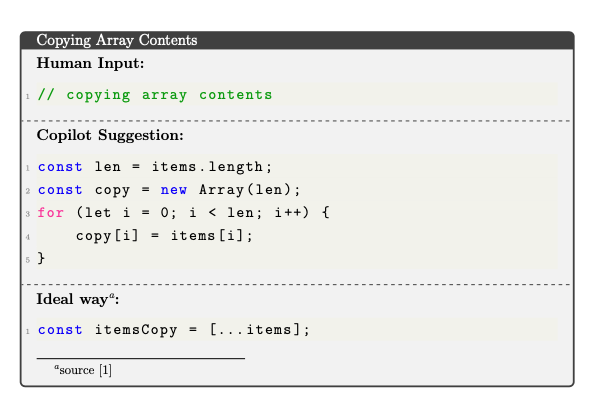
\includegraphics[width=\linewidth]{Figures/bp_1.png}
    \caption{Best Practice for Copying Array Contents amd \cop{} Suggestion.}
    \label{fig:bp_1}
\end{figure}


\section{Chapter Summary}
In summary, we start this chapter by showing the methodology used in addressing textbf{RQ-1} (What are the current boundaries of \cct{}?). 
We first introduced Pythonic idioms and best practices in JavaScript.
We then present our sampling approach for sampling 25 coding scenarios to analyze Copilot code suggestions.
Furthermore, we discussed the input given to Copilot to trigger a code suggestion 
and how the input was restricted to deriving the desired way from the input.
Finally, we described our evaluation approach for Copilot code suggestions.

We sampled 25 Pythonic idioms from Alexandru et al.~\cite{Alexandru2018}, and Farook et al.~\cite{idioms}.
We identified that Copilot did not suggest the idiomatic way as its top suggestion for 23 out of 25 coding scenarios in Python, which addressed \textbf{RQ-1.1} (How do \cct{} manage programming idioms?).
Furthermore, we sampled 25 best practices in JavaScript from the AirBNB JavaScript coding style guide~\cite{airbnb_code}. We identified that Copilot did not suggest the recommended best practice for 22 out of 25 coding scenarios in JavaScript, which addressed \textbf{RQ-1.2} (How do \cct{} manage to manage to suggest non-smelly code?).


% we showed that Copilot struggles to detect and most common idiomatic ways present in public repositories of GitHub and rank them higher than the non-idiomatic ways. The ideal behavior of \cct{} like Copilot in solving this problem is detecting common patterns present in code and rank them higher as the idiomatic ways for a task.
% In the next chapter (chapter~\ref{smells}), we look into how this ideal behavior can cause problems in the case of code smells, where common bad practices present in public repositories of GitHub can make \cct{} like Copilot introduce bad coding practices in its suggestions.

% % \section{Chapter Summary}
% In summary, we start this chapter by showing the methodology used in addressing \textbf{RQ-1.2} (How do \cct{} manage to suggest non-smelly code?). We first introduced the study setup with the input to Copilot and how it was restricted to deriving the best practice from the input and how the suggestions from Copilot were evaluated. We sampled best practices from AirBNB JavaScript coding style guide~\cite{airbnb_code}, and then compared it against Copilot suggestions. Based on results shown in Table~\ref{tab:all_bp}, Copilot struggles to suggest the best practices from widely used coding standards in its suggestions. 

In this chapter, we showed that Copilot struggles to detect and follow coding style guides present in public repositories of GitHub and always suggests code that follows those coding style guides. We also observed that Copilot struggles to detect and most common idiomatic ways present in public repositories of GitHub and rank them higher than the non-idiomatic ways. 
Identifying this delineation could help in urn AI-supported code completion tools such as Copilot into full-fledged AI-supported software engineering tools.
In the next chapter (chapter~\ref{chapter:framework}), we illustrate our taxonomy inspired by autonomous driving levels on the software abstraction hierarchy in \AISE{} and delineate where \cct{} like Copilot currently stands in the taxonomy. 
	\startchapter{Language Idioms and Code Smells}
\label{chapter:idioms}

\section{Introduction}
Useful \AISE{} tools should always suggest the optimal way as its first suggestion. In this chapter, we test if \cop{} suggests the optimal way. 
We begin by explaining our approach to \textbf{RQ-1.2} (How do \cct{} manage programming Idioms and Best Practices?). 

To achieve this, we conduct an exploratory study to find how often does current \cct{} suggest the optimal way in their suggestions. In section~\ref{methodology}, we describe our methodology for the two categories under study: python idioms (Section~\ref{secidioms}) and best practices in javascript (Section~\ref{bp}).
We then compare the suggestions generated by \cop{} and previous works on best practices in Python and JavaScript. We report on how many times \cop{} suggested the optimal way. 

We find that \cop{} performs poorly in suggesting the optimal way in its suggestions. Further, in section~\ref{evolution}, we provide a detailed discussion on how best practices change over time with an example from Asynchronous JavaScript and outline the difficulties of a \cct{} to keep updating its suggestions and reflect the current best practice.

\section{Methodology}
\label{methodology}
In this Section, We explain the methodology we used to address \textbf{RQ-1.2} (How do \cct{} manage programming Idioms and Best Practices?), including how the best practices were sampled (Section~\ref{sampling}), what was the input for copilot (Section~\ref{input}) and how is the suggestion evaluated (Section~\ref{evaluation}). All of the following analysis was carried out using \cop{} extension in Visual Studio Code. We use the most recent stable release of Copilot extension (version number todo) in Visual Studio Code.

\subsection{Sampling Approach}
\label{sampling}
To give the best chance for \cop{} to suggest the optimal way, we sampled the top ten most frequent idioms used in open source projects. So that, \cop{} will have the optimal way more frequently in its training data. However, \cop{} is closed source and we cannot determine if the frequency of code snippet in training data affects \cop{} suggestions in any way. Research by GitHub shows that Copilot can sometimes recite from its training data in ``generic contexts"\footnote{\url{https://github.blog/2021-06-30-github-copilot-research-recitation/}}, which may lead to Licence Infringements shown in Section~\ref{challenges}. Sampling the most frequently used Idioms will also help understand if copilot can recite idioms, which is the ideal behaviour for \cct{}.

\subsection{Study Setup}

\subsubsection{Input to \cop{}}
\label{input}
The input to \cop{} consisted of the idiom title as the first comment to provide context, and the input was restricted to being able to derive the ideal way from the input. This is done to ensure \cop{} is making the decision to suggest the good/bad way in its suggestions. This input style also mimics a novice user, who is unaware of the idioms and useful \cct{} should drive the novice user to use best practices.

\subsubsection{Evaluation}
\label{evaluation}
We considered \cop{} suggested the optimal way if Copilot suggested the best practice in the first suggestion, In this case, we considered \cct{} like \cop{} as productivity tool and user should be saving time as opposed to writing the optimal way without using \cct{}, Scrolling through all the suggestions to deduce the optimal way defeats this purpose. For this reason, We restricted ourselves to first suggestion. However, we do note if the best practice appeared any of the top 10 suggestions currently viewable in \cop{} interface. 

% including sections in other files.
\subsection{Paradigms and Idioms}
Paradigms and idioms are our taxonomy's third level of software abstraction. 
This level requires the code suggested by \cct{} to satisfy all the previous levels of abstractions and use common paradigms and language idioms in its code suggestions. 
These include common practices of solving a programming task. 

Returning to our running example of performing a sorting operation on a list of numbers. 
To satisfy this level of abstraction, \cct{} should suggest a syntactically correct list sorting code, using idiomatic ways in its code suggestions, like the Pythonic way of swapping items in a list~(line 5 in figure~\ref{fig:idioms}), As opposed to suggesting non-idiomatic approaches like creating another temporary variable to swap items in a list shown in correctness level~(figure~\ref{fig:correctness}).

Figure~\ref{fig:idioms} shows the sorting example and the Python code suggestions from \cct{} at this abstraction level.

\begin{figure}[hbt!]
    \centering
\begin{tcolorbox}[title=Idioms level suggestion for sort routine,boxsep=.15mm]
    %https://tex.stackexchange.com/questions/337909/tcolorbox-tcbline-style
\textbf{Human Input:}
\begin{lstlisting}[language={Python}]
# sorting a list
arr = [2,4,1,3,7,5]
\end{lstlisting}
\tcbline
\textbf{\cct{} suggestion:}
\begin{lstlisting}[language={Python}]
n = len(arr)
for i in range(n):
	for j in range(n-1):
		if arr[j] > arr[j+1]:
			arr[j], arr[j+1] = arr[j+1], arr[j]
print(arr)
\end{lstlisting}
\end{tcolorbox}
    \caption{Code suggestion of \cct{} at paradigms and idioms level.}
    \label{fig:idioms}
\end{figure}

The goal of this software abstraction level in the taxonomy is for \cct{} to detect and use commonly known idiomatic approaches and paradigms that occur in public code in its suggestions for suggesting code to solve a programming task.

The capabilities required by \cct{} to satisfy paradigms and idioms level of software abstraction are as follows:
\begin{enumerate}
    \item Identify common patterns like paradigms and language idioms in public code repositories~(training data).
    \item Use paradigms and language idioms in suggesting solutions for a programming task.
    \item Satisfy requirements of all the levels below paradigms and idioms in our taxonomy.
\end{enumerate}


\section{Best Practices}
\label{bp}
A good \AISE{} tool should only suggest code that passes code reviews by humans. Code review problems align with the Code Smell level (middle level) in our taxonomy. 

% For example, in JavaScript, callback api was used in the past to achieve concurrency which were replaced by promises. We checked if Copilot suggests code which is specifically mentioned in the JavaScript documentation as a bad practice or an anti-pattern. Bad Practices in using promises for asynchronous JavaScript like not returning promises after creation, forgetting to terminate chains without catch statement, which are explained in documentation\footnote{\url{https://developer.mozilla.org/en-US/docs/Web/JavaScript/Guide/Using_promises}} and StackOverflow\footnote{\url{https://stackoverflow.com/questions/30362733/handling-errors-in-promise-all/}} are not known to Copilot and suggested code with those common anti-patterns as they occur more frequently in Copilot training data.

\noindent\textbf{Method:} We relied on the AirBNB JavaScript coding style guide~\cite{airbnb_code}, a widely used coding style and code review standard. 
The AirBNB standard contains a variety of best practices. 
We chose practices that were closer to the the design level of our taxonomy, rather than the code level (e.g., logging practices rather than trailing comma use in Javascript). 
We focus on five JavaScript coding standards. % from the AirBNB JavaScript coding style guide~\cite{airbnb_code}. 
The input we gave Copilot consisted of the best practice name as the first comment to provide context, and then minimal extra input to prompt Copilot. 
%The listing \textsf{Copying Array Contents} explains our input, Copilot's suggestion, and the ideal/preferred way. 
% This is to ensure Copilot is making the decision to suggest the good/bad way. 
We considered the suggestion a match if Copilot suggested the ideal way as its first suggestion, under the assumption that most developers would not spend time looking through the remaining nine. We do note if the recommended way appeared any of the top 10 suggestions. 
% Below is the list of five best practices we tested:
% \neil{i think a quick list listing the chosen standards would help, alongside the place the suggestion occurred (e.g.).}

Copilot failed to suggest the recommended way for all five standards we tested, i.e, Copilot did not have the recommended way in its top two suggestions. Only 1 out of 5 standards had the recommended approach in the top 10 suggestions. 

Below is an example of Copying Array Contents (Practice 3). 
We first show the user input that triggers Copilot, the top suggestion by Copilot (i.e., model output) and the recommended way suggested by the AirBNB coding style guide~\cite{airbnb_code}.

\begin{tcolorbox}[title=Copying Array Contents,boxsep=.5mm]
    %https://tex.stackexchange.com/questions/337909/tcolorbox-tcbline-style
\textbf{Human Input:}
\begin{lstlisting}[language=JavaScript]
// copying array contents
const len = items.length;
\end{lstlisting}
\tcbline
\textbf{Copilot Suggestion:}
\begin{lstlisting}[language=JavaScript]
const copy = new Array(len);
for (let i = 0; i < len; i++) {
	  copy[i] = items[i];
}
\end{lstlisting}
\tcbline
\textbf{Ideal way\footnote{source \cite{airbnb_code}}:}
\begin{lstlisting}[language=JavaScript]
const itemsCopy = [...items];
\end{lstlisting}
\end{tcolorbox}
\subsection{Evolution of Best Practices}
\label{evolution}
\section{Chapter Summary}
In summary, we start this chapter by showing the methodology used in addressing \textbf{RQ-1.2} (How do \cct{} manage to suggest non-smelly code?). We first introduced the study setup with the input to Copilot and how it was restricted to deriving the best practice from the input and how the suggestions from Copilot were evaluated. We sampled best practices from AirBNB JavaScript coding style guide~\cite{airbnb_code}, and then compared it against Copilot suggestions. Based on results shown in Table~\ref{tab:all_bp}, Copilot struggles to suggest the best practices from widely used coding standards in its suggestions. 

In this chapter, we showed that Copilot struggles to detect and follow coding style guides  present in public repositories of GitHub and always suggest code that follows those coding style guides. The ideal behavior of \cct{} like Copilot in solving this problem is to detect the coding style guideline from existing code in the project and always suggest code that follows the guideline.

In the next chapter (chapter~\ref{chapter:framework}), we illustrate our taxonomy inspired from autonomous driving levels on the software abstraction hierarchy in \AISE{}, and delineate where \cct{} are currently best able to perform, and where more complex software engineering tasks overwhelm them.
	\startchapter{Framework}
\label{chapter:framework}

\section{Introduction}
In Chapters~\ref{chapter:idioms} and \ref{chapter:smells}, we identified that Copilot does not perform well in detecting and suggesting language idioms and best practices, 
the scope of capability for \cct{} like Copilot is uncertain. In this chapter, we try to address \textbf{RQ-1} (What are the current boundaries of code completion tools) with a taxonomy of 5 software abstraction levels to help access the current capabilities of Copilot. 

We explain each software abstraction level in the taxonomy and the capabilities required by \cct{} to satisfy the software abstraction level. 
We try to delineate where current \cct{} are currently best able to perform, and where more complex software engineering tasks overwhelm them. We use a sorting routine as an example scenario to show how a \cct{} suggestion looks like at every level of abstraction in our taxonomy.

\subsection{Motivation}
To center our analysis on creating a software abstraction hierarchy, we leverage an analogous concept in the more developed (but still nascent) field of autonomous driving. 
Koopman has adapted the SAE Autonomous Driving safety levels~\cite{sae} to those shown in figure~\ref{fig:koopman_pyramid}. 
The pyramid concept is derived from that of Maslow~\cite{Maslow1943}, such that addressing aspects on the top of the pyramid first require the satisfaction of aspects below. 
For example, before being able to think about system safety (such as what to do in morally ambiguous scenarios), the vehicle must first be able to navigate its environment reliably (``Basic Driving Functionality'').

We think that a similar hierarchy exists in \AISE{}. Before worrying about software architecture issues, that is, satisfying system quality attributes such as performance, \AISE{} tools need to be able to exhibit ``basic programming functionality''. This basic functionality is where most research effort is currently concentrated, such as program synthesis, \cct{}, and automated bug repair.

\begin{figure}[hbt!]
    \centering
    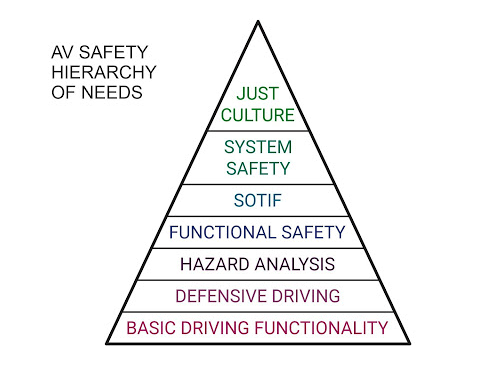
\includegraphics[width=.8\linewidth]{Figures/koopman_pyramid.png}
    \caption{Koopman's Autonomous Vehicle Safety Hierarchy of Needs~\cite{koopman}. SOTIF = safety of the intended function.}
    \label{fig:koopman_pyramid}
\end{figure}

\section{Taxonomy}
\label{taxonomy}
Our taxonomy is a software abstraction hierarchy where ``basic programming functionality'' such as code compilation and syntax checking is the lowest abstraction level,
Software architecture analysis and design is the highest abstraction level.
As we ascend the levels, just as with Koopman's pyramid in figure \ref{fig:koopman_pyramid}, 
software challenges rely more on human input and become more difficult to automate (e.g., crafting design rules vs following syntax rules).

Figure~\ref{fig:taxonomy} shows the taxonomy of autonomy levels for \cct{}.  The more abstract top levels depend on resolution of lower ones. As we move up the hierarchy, we require more human oversight of the AI; as we move down the hierarchy, rules for detecting problems are easier to formulate. Green levels are areas where \cct{} like Copilot works reasonably well, while red levels are challenging for Copilot as shown in chapters~\ref{chapter:idioms} and~\ref{chapter:smells}.

\begin{figure}[hbt!]
    \centering
    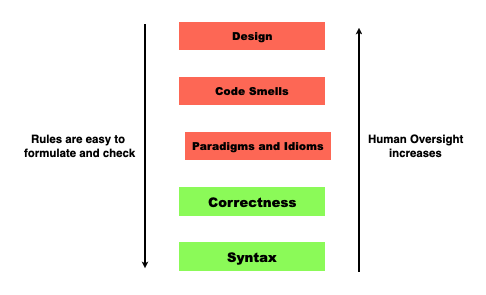
\includegraphics[width=\linewidth]{Figures/taxonomy.png}
    \caption{Hierarchy of software abstractions.}
    \label{fig:taxonomy}
\end{figure}

The challenges further up the hierarchy are nonetheless more important for software quality attributes (QA)~\cite{Ernst2017} and for a well-engineered software system.
For example, an automated solution suggested by \cct{} to the top level of the taxonomy would be able to follow heuristics to engineer a well designed software system, one which would be easy to modify and scale to sudden changes in use.
\subsection{Syntax Level}
\label{syntax}
The syntax level is the lowest abstraction level in our taxonomy. This level includes the most basic programming functionality like syntax and code compilations. This level does not require the \cct{} suggested code to successfully perform the task but to suggest code without any obvious errors like syntax errors.
For example, consider a task of perform a sorting operation on a list of numbers. To satisfy this level of abstraction, \cct{} should suggest code that is syntactically correct without any compilation errors and the code is not required to perform the sorting operation correctly. 
Figure~\ref{fig:syntax} shows the example and syntax suggestions from \cct{} at this abstraction level.

\begin{figure}[hbt!]
    \centering
    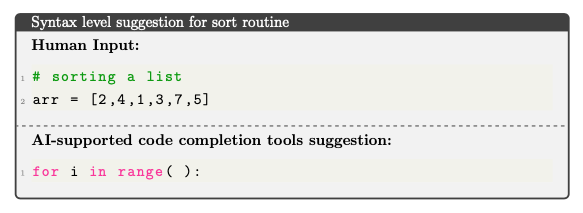
\includegraphics[width=\linewidth]{Figures/syntax.png}
    \caption{\cct{} syntax level suggestions}
    \label{fig:syntax}
\end{figure}

The goal of this software abstraction level in our taxonomy is for a \cct{} to be able to suggest code without any syntactical errors.
The capabilities required by a \cct{} to satisfy this level of abstraction are as follows:

\begin{enumerate}
    \item Suggested code should not produce any errors in code compilation.
    \item Suggested code should be syntactically correct.
\end{enumerate}

% \begin{tcolorbox}[title=Syntax level suggestion for sort routine,boxsep=.15mm]
%     %https://tex.stackexchange.com/questions/337909/tcolorbox-tcbline-style
% \textbf{Human Input:}
% \begin{lstlisting}[language={Python}]
% # sorting a list
% arr = [2,4,1,3,7,5]
% \end{lstlisting}
% \tcbline
% \textbf{\cct{} suggestion:}
% \begin{lstlisting}[language={Python}]
% for i in range( ):
% \end{lstlisting}
% \end{tcolorbox}
\section{Correctness}
\subsection{Idioms}
The paradigms and idioms is the mid level of abstraction in our taxonomy. This level requires the suggested code satisfy syntax and correctness level and use common language idioms in its suggestions. 

For example, considering the task of sorting operation on a list of numbers, to satisfy this level of abstraction, \cct{} should suggest a syntactically correct list sorting code, using a well know algorithm like quick sort or bubble sort. The main goal of this level in the taxonomy is for a \cct{} to be able to use the current best practices and algorithms in its suggestions.

The capabilities required by a \cct{} to satisfy this level of abstraction are as follows
\begin{enumerate}
    \item Satisfy requirements of syntax and correctness level
    \item Use well know algorithms, best practices, and language idioms whenever possible in suggesting a solution for a problem.
\end{enumerate}
\subsection{Code Smells}
The code smells level is the penultimate level of abstraction in our taxonomy, This level requires the suggested code satisfy all the previous levels of abstraction and avoid code smells in its suggestions.

For example, considering the task of  a task of perform a sorting operation on a list of numbers, to satisfy this level of abstraction, AI-supported code completion tools should
suggest a syntactically correct list sorting code, which follows the best practices like using appropriate datatype and variable to store the list.

The capabilities required by a AI-supported code completion tools to satisfy this
level of abstraction are as follows
\begin{enumerate}
    \item Satisfy requirements of syntax and correctness level.
    \item Suggest a solution that does not have any common code smells found in public code repositories.
\end{enumerate}
\subsection{Design}
\label{design}
The top level in our taxonomy is Design, This level requires the suggested code satisfy all the previous levels of abstractions and suggest appropriate design practices for a given input in its suggestions.

For example, considering the task of sorting operation on a list of numbers, to satisfy this level of abstraction, \cct should suggest a syntactically correct list sorting code, using a algorithm which gives the best performance for that scenario like suggesting quick sort instead of bubble sort if it is a large set of numbers. The main goal of this level in the taxonomy is for a \cct{} to be able to pick the algorithms as per given scenario in its suggestions.

\subsubsection{Design Patterns}
\label{patterns}
To satisfy design level \cct{} must be able to capture design and module level concerns. 
These include recapturing design patterns (such as Observer) and architectural tactics (such as Heartbeat) to improve and personalize suggestions. 
To do this, however, the training data must also use these patterns and best practices.
The vision is for something like Copilot to be capable of suggesting patterns like Model-View-Controller (MVC) when prompted. 

The capabilities required by a \cct{} to satisfy this level of abstraction are as follows
\begin{enumerate}
    \item Identify design and module level concerns in code files.
    \item Suggest design patterns and architectural tactics when prompted.
    \item Picking and suggesting the best applicable algorithm for a given scenario.
    \item Satisfy requirements of all previous levels of abstractions.
\end{enumerate}

% \begin{tcolorbox}[title=Code smells level suggestion for sort routine,boxsep=.15mm]
%     %https://tex.stackexchange.com/questions/337909/tcolorbox-tcbline-style
% \textbf{Human Input:}
% \begin{lstlisting}[language={Python}]
% # sorting a list
% arr = [2,4,1,3,7,5]
% \end{lstlisting}
% \tcbline
% \textbf{\cct{} suggestion:}
% \begin{lstlisting}[language={Python}, morekeywords={False, True}]
% swapped = False
% for i in range(len(arr)-1, 0, -1):
% 	for j in range(n):
% 		if arr[j] > arr[j+1]:
% 		    swapped = True
% 			arr[j], arr[j+1] = arr[j+1], arr[j]
% 	if not swapped:
% 	    break
% print(arr)
% \end{lstlisting}
% \end{tcolorbox}
\section{Chapter Summary}

	\startchapter{Discussion, Limitations \& Implications}
\label{chapter:discussion}

\section{Introduction}
Further, in section~\ref{evolution}, we provide a detailed discussion on how best practices change over time with an example from Asynchronous JavaScript and outline the difficulties of a \cct{} to keep updating its suggestions and reflect the current best practice.


\section{Limitations}

\section{Ethical Considerations}
\section{Explainability}
\label{explain}
\cop{} is closed source, and it is currently not possible to determine the source or the reason behind each suggestion, making it difficult to detect any problems (access is only via an API). 
However, engineering software systems is laden with ethical challenges, and understanding why a suggestion was made, particularly for architectural questions such as system fairness, is essential. 
Probes, as introduced in \cite{karmakar21}, might expand technical insight into the models.

Another challenge is understanding the basis for the ranking metric for different suggestions made by Copilot. This metric has not been made public. Thus, we cannot determine the reason Copilot is ranking one approach (e.g., non-idiomatic) over the idiomatic (preferred) approach. However, large language model suggestions are based on its training data~\cite{training_extraction}, so one explanation is that the non-idiomatic approach is more frequent in the training data~\cite{stochastic_parrots}. Better characterization of the rankings would allow users to better understand the motivation. 
\section{Control}
\label{control}
Being generative models, tools like Copilot are extremely sensitive to input with stability challenges and to make them autonomous raises control concerns.
For example, if a human asks for a N\textsuperscript{2} sorting algorithm, should Copilot recommend one, or the NlogN alternative? 
Ideally, tools should warn users if prompted to suggest sub-optimal code. 
\AISE{} should learn to differentiate between optimal and sub-optimal code. 
One direction to look at is following commit histories of files, as they are the possible places to find bug fixes and performance improvements.

\section{Future Directions}
\label{future}
To solve complex software engineering challenges with AI, machine learning models must be able to capture design and module level concerns. 
These include recapturing design patterns (such as Observer) and architectural tactics (such as Heartbeat) to improve and personalize suggestions. 
To do this, however, the training data must also use these patterns and best practices.
The vision is for something like Copilot to be capable of suggesting patterns like Model-View-Controller (MVC) when prompted. 
Being able to identify where design artifacts occur in the code, such as with pattern recovery~\cite{Keim2020}, is one avenue to explore. 
\section{Chapter Summary}
	\startchapter{Conclusion}
\label{conclusion}
GitHub's Copilot and related large language model approaches to code completion are promising steps in \AIDE{}. Software systems need more than development and coding effort, however. 
These systems require complex design and engineering work to build. 
We showed that while the coding syntax and warnings level of software problems is well on its way to useful AI support, the more abstract concerns, such as code smells, language idioms, and design rules, are far from solvable at present.
% The paper explored some potential implications and ways forward for addressing these higher abstraction concerns. 
Although far off, we believe \AISE{}, where an AI supports designers and developers in more complex software \emph{engineering} tasks, is possible.
% API driven development for recommendations 
% 	\appendix
% 	\startappendix{Appendix}
\label{chapter:appendix}




% The style of bibliography exemplified here is the "plain",
% normally used in science theses. This is shown
% by the entry {plain} below. Substitute the
% appropriate bibliography style. See also the
% PDF file "InformationOnBibliographyStyles" in this
% directory for more choices.

% The Bibliography file is a BibTex file named
% UVicThesis.bib and called below

	\TOCadd{Bibliography}
	\bibliographystyle{plain}
	\bibliography{UvicThesis}

\end{document}
